%%% demothesis.tex --- 
%% 
%% Filename: demothesis.tex
%% Description: 
%% Author: Ola Leifler
%% Maintainer: 
%% Created: Thu Oct 14 12:52:20 2010 (CEST)
%% Version: $Id$
%% Version: 
%% Last-Updated: Wed Jun 28 10:57:24 2017 (+0200)
%%           By: Ola Leifler
%%     Update #: 169
%% URL: 
%% Keywords: 
%% Compatibility: 
%% 
%%%%%%%%%%%%%%%%%%%%%%%%%%%%%%%%%%%%%%%%%%%%%%%%%%%%%%%%%%%%%%%%%%%%%%
%% 
%%% Commentary: 
%% 
%% 
%% 
%%%%%%%%%%%%%%%%%%%%%%%%%%%%%%%%%%%%%%%%%%%%%%%%%%%%%%%%%%%%%%%%%%%%%%
%% 
%%% Change log:
%% 
%% 
%% RCS $Log$
%%%%%%%%%%%%%%%%%%%%%%%%%%%%%%%%%%%%%%%%%%%%%%%%%%%%%%%%%%%%%%%%%%%%%%
%% 
%%% Code:

\documentclass[msc,lith,english]{liuthesis}
%% Settings go in settings.tex
\include{settings}
\usepackage{rotating}
\usepackage{eurosym}
\usepackage{color}
\usepackage{hyperref}
\usepackage{listings}
\usepackage{amssymb}
\lstset{
    escapeinside={(*}{*)}
}

% \usepackage{changebar}

%\department{Institutionen för datavetenskap}
%\departmentenglish{Department of Computer and Information Science}
%\departmentshort{IDA}
\department{Institutionen för Systemteknik}
\departmentenglish{Department of Electrical Engineering}
\departmentshort{ISY}

\supervisor{Harald Nautsch}
\examiner{Ingemar Ragnemalm}
\titleenglish{Evaluation of an Appearance-Preserving Mesh Simplification Scheme for Configura AB}
\titleswedish{}
\thesissubject{Computer Graphics and Visualization}

\publicationyear{2018}
\currentyearthesisnumber{001}
\dateofpublication{2018-01-01}

\author{Rasmus Hedin}

\begin{document}

\chapterstyle{VZ43}

%%% intro.tex --- 
%% 
%% Filename: intro.tex
%% Description:
%% Author:
%% Maintainer:
%% Created:
%% Version:
%% Last-Updated:
%%           By:
%%     Update #:
%% URL:
%% Keywords:
%% Compatibility:
%% 
%%%%%%%%%%%%%%%%%%%%%%%%%%%%%%%%%%%%%%%%%%%%%%%%%%%%%%%%%%%%%%%%%%%%%%
%% 
%%% Commentary:
%% 
%% 
%% 
%%%%%%%%%%%%%%%%%%%%%%%%%%%%%%%%%%%%%%%%%%%%%%%%%%%%%%%%%%%%%%%%%%%%%%
%% 
%%% Change log:
%% 
%% 
%% RCS $Log$
%%%%%%%%%%%%%%%%%%%%%%%%%%%%%%%%%%%%%%%%%%%%%%%%%%%%%%%%%%%%%%%%%%%%%%
%% 
%%% Code:


\chapter{Introduction} \label{cha:introduction}
The rendering of meshes (a collection of polygons describing a surface) is one of the main activities in computer graphics (usually, a collection of meshes; a so called scene description). In many cases, these meshes are very detailed, and require a large amount of polygons to fully describe a surface. This is problematic, since the rendering time of a scene depends on the number of polygons it has. Therefore, it is important to reduce the number of polygons in a mesh as much as possible. This is especially true in video games, where the scene needs to be rendered in real-time. However, if the number of polygons are reduced too much, it will degrade the visual quality of a mesh, giving a progressively flatter surface than intended and removing small surface details. This destroys the intended \emph{geometrical appearance} of the mesh.


\section{Motivation} \label{sec:motivation}
While the geometrical appearance of a mesh is important, it is not the only factor which gives the final appearance of a mesh when rendering. According to \emph{Cohen et al.}~\cite{cohen1998appearance}, both the surface curvature and color are equally as important contributors. \emph{Textured appearance} will be used as the common name for these since surface properties are usually specified with a texture map.

In computer graphics, the process to reduce the number of polygons in a mesh based on some metric is called a \emph{mesh simplification algorithm}, as seen in \emph{Talton's survey}~\cite{talton2004short} in the field. Historically, these have been mostly concerned with minimizing the geometrical deviation of a mesh when applying it. Somewhat recently, methods for minimizing the texture deviation when simplifying a mesh have also appeared. They attempt to reduce the texture deviation and stretching caused when removing polygons from a mesh, as described in \emph{Hoppe et al.}~\cite{hoppe1996progressive}.

By simultaneously taking into account the geometrical and texture deviation, one can preserve the \emph{visual appearance} of a mesh when simplifying it. If polygons can be removed without affecting this appearance significantly, the rendering time can be reduced for ``free''.

\section{Aim} \label{sec:aim}
The aim of this thesis is to first perform a literature study of mesh simplification algorithms that preserve the visual appearance of a mesh. A suitable solution will then be integrated as a preprocessing step in \emph{CET Designer's} graphics pipeline. CET Designer is a space planning software developed by the company \emph{Configura AB} (see \cref{sec:background} for a more detailed description). Considering the visual appearance when simplifying a mesh will enable Configura to generate better \emph{Level of Detail} (LoD) meshes for speeding up their rendering time. Currently, Configura only takes the geometrical deviation into account when simplifying, with no regard for the textures (e.g. diffuse or normal) on top of the mesh.


\section{Research Questions} \label{sec:research-questions}
\begin{enumerate}
\item What alternative \emph{mesh simplification schemes} exist that \emph{preserves the appearance} of a mesh? 
\item Which of these alternatives would be appropriate to integrate into Configura's software?
\end{enumerate}

\section{Delimitations} \label{sec:delimitations}
Since the thesis is done on a time limit a comparison of multiple mesh simplification schemes taking the appearance into account is not feasible. Therefore, one mesh simplification algorithm will be chosen to be implemented and evaluated. The choice will be based on a study of algorithms that can be found in the literature.

\section{Background} \label{sec:background}
This thesis was requested by Configura AB, a company in Linköping which provides space planning software. Their main product, \emph{CET designer}, lets companies plan, create, and render 3-D spaces (among other things). These scenes can have a large amount of polygons that need to be rendered in real-time for customers to evaluate their creations in CET designer. 

To allow larger scenes to be rendered with higher frame-rates (e.g. needed when exploring environments in \emph{Virtual Reality} (VR), to prevent motion sickness), it would be beneficial to reduce the amount of polygons as much as possible. The meshes in these scenes usually have textures applied to them, and it is therefore important to keep the quality as high as possible.

While Configura already has a mesh simplification in their pipeline, it only accounts for surface simplifications, and does not take into account the texture appearance that might be degraded when applying mesh simplification. Hence, the given task was to integrate a new mesh simplification scheme that takes into account texture quality when simplifying a mesh.

%%%%%%%%%%%%%%%%%%%%%%%%%%%%%%%%%%%%%%%%%%%%%%%%%%%%%%%%%%%%%%%%%%%%%%
%%% intro.tex ends here

%%% Local Variables: 
%%% mode: latex
%%% TeX-master: "thesis"
%%% End: 

%%% lorem.tex --- 
%% 
%% Filename: lorem.tex
%% Description: 
%% Author: Ola Leifler
%% Maintainer: 
%% Created: Wed Nov 10 09:59:23 2010 (CET)
%% Version: $Id$
%% Version: 
%% Last-Updated: Tue Oct  4 11:58:17 2016 (+0200)
%%           By: Ola Leifler
%%     Update #: 7
%% URL: 
%% Keywords: 
%% Compatibility: 
%% 
%%%%%%%%%%%%%%%%%%%%%%%%%%%%%%%%%%%%%%%%%%%%%%%%%%%%%%%%%%%%%%%%%%%%%%
%% 
%%% Commentary: 
%% 
%% 
%% 
%%%%%%%%%%%%%%%%%%%%%%%%%%%%%%%%%%%%%%%%%%%%%%%%%%%%%%%%%%%%%%%%%%%%%%
%% 
%%% Change log:
%% 
%% 
%% RCS $Log$
%%%%%%%%%%%%%%%%%%%%%%%%%%%%%%%%%%%%%%%%%%%%%%%%%%%%%%%%%%%%%%%%%%%%%%
%%
%%% Code:


\chapter{Theory} \label{ch:theory}
Since several mesh simplification algorithms are being considered, \cref{sec:related_work} gives a brief overview of the most notable schemes found in previous work. A more detailed explanation of the algorithms can be found in \cref{sec:appearance-preserving_simplification,sec:quadric-based_error_metric,sec:progressive_meshes}.

Afterwards, in \cref{sec:metrics_for_appearance_preservation}, the different metrics that can be used to measure the appearance preservation after a simplification has been done is discussed. This will later be used to evaluate the solution empirically by giving a concrete metric for the amount of appearance deviation.

Finally, in \cref{sec:measuring_algorithmic_performance}, the methods and common practices for measuring performance of an algorithm are discussed. Based on existing industry practices, we show how to measure the computation time and memory usage of the algorithms. Since these measurements can be noisy, statistical methods will need to be used to truthfully answer our research questions.

%%%%%%%%%%%%%%%%%%%%%%%%%%%%%%%%%%%%%%%%%%%%%%%%%%%%%%%%%%%%%%%%%%%%%%
%%
%%% Related Work
%%
%%%%%%%%%%%%%%%%%%%%%%%%%%%%%%%%%%%%%%%%%%%%%%%%%%%%%%%%%%%%%%%%%%%%%%
\section{Related Work} \label{sec:related_work}
Some different approaches have been presented in the literature to solve the problem of simplifying a mesh. Early solutions focused on the geometrical error which is enough in many cases, but in the case of a mesh with appearance attributes this may give a poor result. Other solutions have been presented that takes the attributes into account to give a better appearance of the mesh. This section will give a brief overview of the simplification algorithms that can be found in the literature.

According to \emph{David Luebke's survey}~\cite{luebke2001developer} on the subject, mesh simplification is a technique which transforms a geometrically complex mesh (with a lot of polygons) to a simpler representation by removing unimportant geometrical details (reducing the number of polygons). It does this by assuming that some meshes are small, distant, or have areas which are unimportant to the visual quality of the rendered image. For example, if the camera in a scene always faces toward a certain direction, then removing details from the backside of a mesh won't affect the final rendered result, since they will never be seen by the camera anyway. Reducing the number of polygons allows meshes to use less storage space and need less computation time.

There are many mesh simplification algorithms, as can be seen in \emph{David Luebke's survey}~\cite{luebke2001developer}, each presenting a new approach with their own strengths and weaknesses. The first scheme is due to \emph{Schroeder et al.}~\cite{schroeder1992decimation} in 1992, called \emph{mesh decimation}. It was meant to be used to simplify meshes produced by the marching cubes algorithm, which usually gives unnecessary details. It works by making multiple passes through the meshes' vertices, and deleting vertices that do not destroy local topology and are within a given distance threshold when re-triangulated.

Besides \emph{decimation-based methods}, such as the aforementioned mesh decimation scheme, there exists another class of simplifiers based on \emph{vertex-merging mechanisms}. According to \emph{Luebke}~\cite{luebke2001developer}, these work by iteratively collapsing a pair of vertices \((v_j, v_k)\) into a single vertex \(v_i\). This will also remove any polygons which were suspended by \((v_j, v_k)\). The first collapse scheme is due to \emph{Hoppe et al.}~\cite{hoppe1993mesh}, which shows an \emph{edge collapse} of \(e_{ji} = (v_j, v_i) \rightarrow v_i\) as in \cref{fig:mesh_transformations} (a). There exist other schemes, such as \emph{pair contraction} in \cref{fig:mesh_transformations} (c) where vertices within a distance $t$ are allowed to be merged. These don't tend to preserve the local topology of the original mesh, and instead focus on a more aggressive simplification.

\begin{figure}[h]
    \centering
    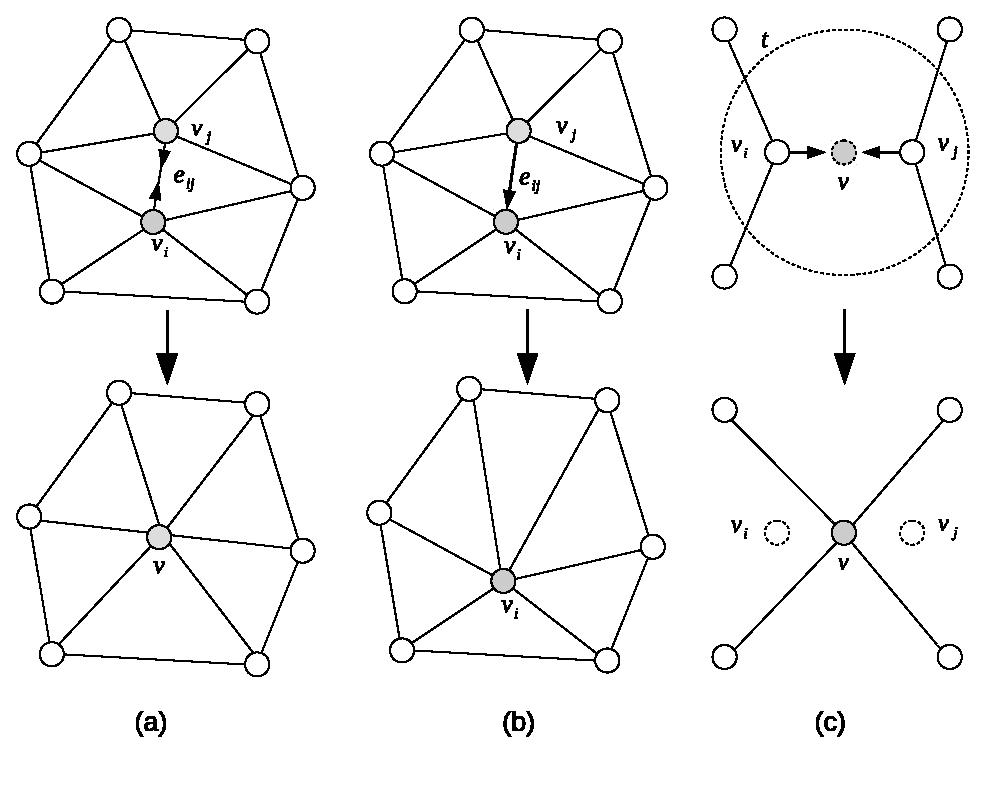
\includegraphics[width=\textwidth]{figures/mesh_transformations.eps}
    \caption{(a) edge collapse, (b) vertex removal, and (c) pair contraction}
    \label{fig:mesh_transformations}
\end{figure}

\emph{Quadric Error Metrics} (QEM), due to \emph{Garland and Heckbert} \cite{garland1997surface} performs edge collapses to provide a provably optimal simplification. In each iteration, an edge is collapsed \((v_j, v_i) \rightarrow \mathbf{v}\) and \(\mathbf{v}\) is repositioned at the position which gives the lowest possible geometrical error. \emph{Hoppe} \cite{hoppe1996progressive} also perform edge collapses but he tries to minimize an energy function. The edge with the lowest estimated energy is chosen for the collapse. 


%\subsection{Preserving appearance}
Focusing on minimizing the geometrical error during simplification works well for many meshes. But in the case of a mesh with appearance attributes such as color, normals, and texture coordinates the result may be poor. A common way to solve this is to use a metric which does not only take the geometry, but also the appearance attributes into account.

\emph{Cohen et al.} \cite{cohen1998appearance} defines a new \emph{texture deviation metric} which takes three attributes into account: Surface position, surface curvature, and surface color. These attributes are sampled from the input surface and the simplification is done with edge collapses and vertex removals.

\emph{Sander et al.} \cite{sander2001texture} uses the texture deviation metric together with a \emph{texture stretch metric} to better balance frequency content in every direction all over the surface.

An extended more general version of the QEM is presented by \emph{Garland and Heckbert} \cite{garland1998simplifying} where the metric can be used for points in $n$-dimensional space. Thus, when the color is considered each vertex would be represented by a 6-dimensional vector. Another version of QEM by \emph{Hoppe} \cite{Hoppe:1999:NQM:319351.319357} base the attribute error on geometric correspondence in 3D rather than using points in $n$-dimensional space.

\emph{Image-driven simplification} defined by \emph{Lindstrom and Turk} \cite{lindstrom2000image} captures images from different angles of the mesh. The distance between images of the mesh before and after an edge collapse are used to guide the simplification.

\iffalse %%%%%%%%%%%%%%%%%%%%%

============================
 Mesh simplification
============================
* Geometry
  - Mesh decimation
  - Mesh optimization
  - Progressive meshes
  - Surface simplification using quadric error metric
  
* Geometry and appearance attributes
  - Appearance-preserving simplification

  - Texture mapped progressive meshes
  
  - Simplifying surfaces with color and texture using quadric error metric
  - New quadric error metric

  - Image-driven simplification

============================
 Mesh parametrization
============================
  Resample texture
  Ray tracing
  Volume UV
  
\fi %%%%%%%%%%%%%%%%%%%%%%%%%%
  
\iffalse %%%%%%%%%%%%%%%%%%%%%
\section{Mesh Transformations} \label{sec:mesh_transformations}
The detail of a mesh can be reduced/increased by altering the vertices and edges of the mesh. There exist several mechanisms that can be used.

\begin{itemize}
\item Edge collapsing
\item Vertex removal
\item Pair contraction
\item Vertex split
\end{itemize}

In edge collapsing, the vertices of the edge $e_{ij} = (v_i, v_j)$ is removed and replaced with a single vertex $v$ somewhere in between. The triangles that used the edge $e_{ij}$ is removed and the neighbors of $v_i, v_j$ will be connected with the new created vertex. This can be seen in \cref{fig:mesh_transformations}(a).

Vertex removal is similar to edge collapsing, but now only one vertex is removed and the other vertex is moved to the location of the removed vertex. The neighbors of the removed vertex will be connected to the one that remains. In ~\cref{fig:mesh_transformations}(b) vertex $v_j$ of edge $e_{ji}$ is removed and vertex $v_i$ is moved to the location of $v_j$.

In a pair contraction, it is possible to merge two distant vertices that are not connected by an edge. Usually, the vertices have to within a certain threshold to be considered for a contraction. In \cref{fig:mesh_transformations}(c) the vertices $v_j, v_k$ is contracted into the new vertex $v_i$. 

To increase the detail of the mesh an existing vertex can be split into two, i.e. vertex split. When performing a vertex split a vertex $v$ is split into two new vertices $v_i, v_j$ connected by an edge $e_{ij}$. 

\begin{figure}[h]
    \centering
    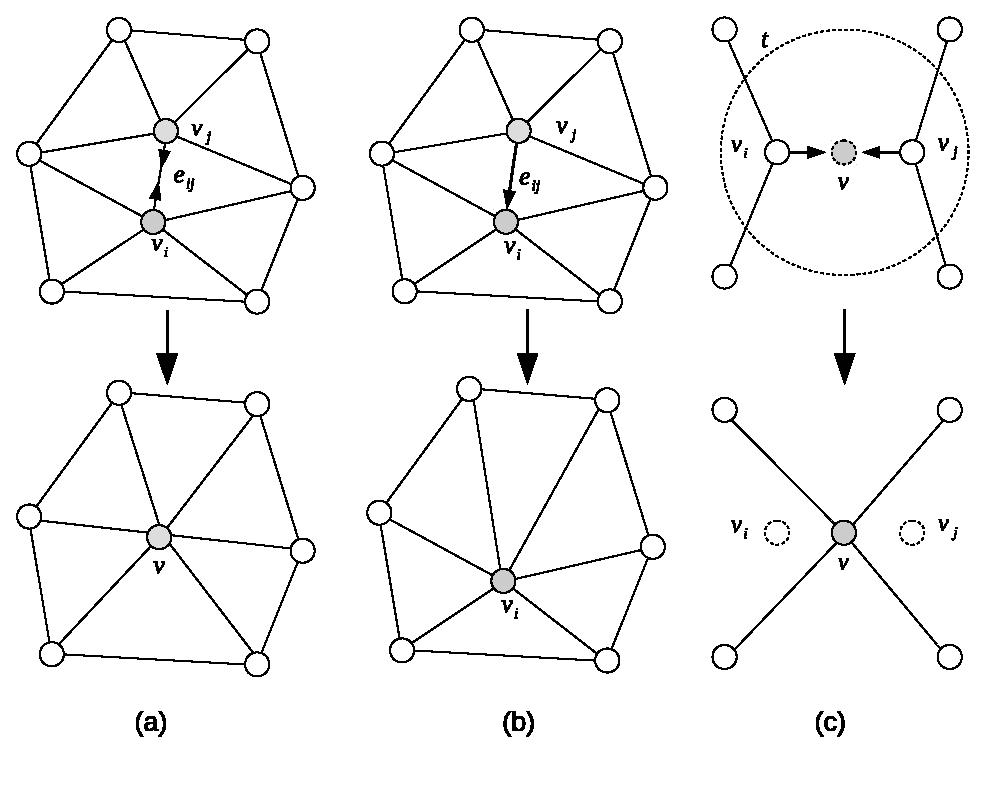
\includegraphics[width=\textwidth]{figures/mesh_transformations.eps}
    \caption{(a) edge collapse, (b) vertex removal, and (c) pair contraction}
    \label{fig:mesh_transformations}
\end{figure}
\fi %%%%%%%%%%%%%%%%%%%%%%%%%%

%%%%%%%%%%%%%%%%%%%%%%%%%%%%%%%%%%%%%%%%%%%%%%%%%%%%%%%%%%%%%%%%%%%%%%
%%
%%% Appearance-Preserving simplification
%%
%%%%%%%%%%%%%%%%%%%%%%%%%%%%%%%%%%%%%%%%%%%%%%%%%%%%%%%%%%%%%%%%%%%%%%
\section{Appearance-Preserving Simplification} \label{sec:appearance-preserving_simplification}
In order to preserve the appearance of a model when it is simplified, \emph{Cohen et al.} \cite{cohen1998appearance} defines a \emph{texture deviation metric}. This metric takes three attributes into account: Surface position, surface curvature, and surface color. To properly sample these attributes from the input surface, the surface position is decoupled from the color and normals stored in texture and normal maps, respectively. The metric guarantees that the maps will not shift more than a user-specified number of pixels on the screen. This user-specified number is defined as $\epsilon$.

Approximation of the surface position is done offline with simplification operations such as edge collapsing and vertex removals. At run-time, the color and normals are sampled in pixel-coordinates with mip-mapping techniques. Mip-maps are a pre-calculated sequence of images with progressively lower resolution. Here the decoupled representation is useful since the texture deviation metric can be used to bound how much the mapped attributes value's positions deviate from the positions of the original mesh. This guarantees that the sampling and mapping to screen-space of the attributes is done in an appropriate way.

Before any simplification can be made, a parametrization of the surface is required in order to store the color and normals in maps. If the input mesh does not have a parametrization, it is created and stored per-vertex in texture and normal maps. Next, the surface and maps are fed into the simplification algorithm which decides which simplification operations to use and in what order. The deviation caused by each operation is measured with the texture deviation metric. A \emph{progressive mesh} (PM) with error bounds for each operation is returned by the algorithm, which can then be used to create a set of LOD with error bounds. Using the error bounds, the tessellation of the model can be adjusted to meet the user-specified error $\epsilon$.

%%%%%%%%%%%%%%%%%%%%%%%%%%%%%%%%%%%%%%%%%%%%%%%%%%%%%%%%%%%%%%%%%%%%%%
%%
%%% Quadric-Based Error Metric
%%
%%%%%%%%%%%%%%%%%%%%%%%%%%%%%%%%%%%%%%%%%%%%%%%%%%%%%%%%%%%%%%%%%%%%%%
\section{Quadric-Based Error Metric} \label{sec:quadric-based_error_metric}
% Surface simplification using quadric error metric
\iffalse %%%%%%%%
\begin{figure}[ht]
    \centering
    \begin{minipage}{0.49\textwidth}
        \centering
        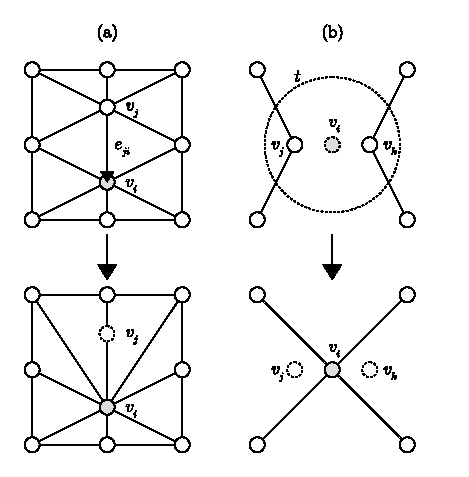
\includegraphics[width=\textwidth]{figures/contraction_types.eps}
        \caption{(a) edge \(e_{ji} = (v_j, v_i)\) contraction toward \(v_i\)
                 and (b) pair \((v_j, v_k)\) contraction in the distance threshold \(t\) toward new vertex \(v_i\).}
        \label{fig:contractions}
    \end{minipage} \hfill
    \begin{minipage}{0.485\textwidth}
        \centering
        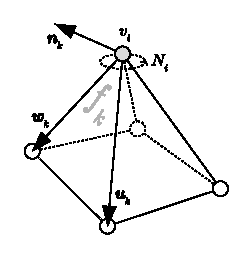
\includegraphics[width=\textwidth]{figures/quadric_planes.eps}
        \caption{Depiction of one of the planes \(f_k\) in the neighborhood \(N_i\) of the vertex \(v_i\). It has a normal \(\mathbf{n}_k\); found by the \(\mathbf{w}_k \times \mathbf{u}_k\) of its edges.}
        \label{fig:quadrics}
    \end{minipage}
\end{figure}
\fi %%%%%%%%%

Mesh simplification with \emph{Quadric Error Metrics} (QEM), due to \emph{Garland and Heckbert}~\cite{garland1997surface}, is based on the vertex merging paradigm. It provides a provably optimal simplification in each iteration, by collapsing the edge \((v_j, v_i) \rightarrow v_i\) and re-positioning it at \(\mathbf{v}\), which gives it the lowest possible geometrical error. By assigning a matrix \(\mathbf{Q}_i\) for each vertex \(v_i\), one can find the error \(\mathup\Delta(\mathbf{v})\) introduced by moving \(v_i\) to \(\mathbf{v}\). \(\mathup\Delta(\mathbf{v})\) is the sum of squared distances from \(\mathbf{v}\) to the planes \(\mathbf{f}_k\) in \(v_i\)'s neighborhood \(N_i\) (all polygons around \(v_i\) as in \cref{fig:quadrics}).

\begin{figure}[ht]
  \centering
  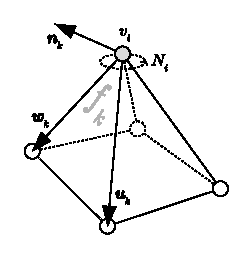
\includegraphics[width=0.4\textwidth]{figures/quadric_planes.eps}
  \caption{Depiction of one of the planes \(f_k\) in the neighborhood \(N_i\) of the vertex \(v_i\). It has a normal \(\mathbf{n}_k\); found by the \(\mathbf{w}_k \times \mathbf{u}_k\) of its edges.}
  \label{fig:quadrics}
\end{figure}

%\vspace{-0.7em}

Since \(\mathup\Delta(\mathbf{v})\) is quadratic, finding a \(\mathbf{v}\) which gives a minimal error is a linear problem. The best position \(\mathbf{\overline{v}}_i\) for \(v_i\) after a collapse \((v_j, v_i) \rightarrow v_i\) is a solution to \cref{eq:quadric_opt}.

\begin{equation} \label{eq:quadric_opt}
(\mathbf{Q}_j + \mathbf{Q}_i)\mathbf{\overline{v}}_i = \begin{bmatrix} 0 & 0 & 0 & 1 \end{bmatrix}\transpose.
\end{equation}

\begin{equation} \label{eq:homogeneous_quadric}
      \mathup\Delta(\mathbf{v}) = \mathbf{v}\transpose \mathbf{Q}_i  \mathbf{v} \;,\;\; \mathbf{Q}_i = \sum_{f_k \in N_i}  \mathbf{f_k} \mathbf{f_k}\transpose \; .
\end{equation}

By storing the \(\mathup\Delta(\mathbf{\overline{v}}_i)\) for every valid collapse \((v_j, v_i) \rightarrow v_i\) in a min-heap, the least cost collapse on the top of the heap can be done in each iteration, removing a vertex in each step. This is repeated until either a user-given vertex count \(|\mathcal{V}|\) is reached or until some error threshold \(\epsilon\).

The results by \emph{Garland and Heckbert}~\cite{garland1997surface} show that QEM can reduce the simplification error by up to 50 \% in comparison to a na\"ive scheme where \(\mathbf{\overline{v}}_i = (v_i + v_j) / 2\) and \(\Delta(\mathbf{\overline{v}}_i) = ||\mathbf{\overline{v}}_i - v_i||\). They also argue that QEM gives higher-quality simplifications than \emph{vertex clustering} and that it is faster than \emph{progressive meshing} (which we also present later).

\iffalse
\begin{figure}[ht]
    \centering
    \includegraphics[width=\textwidth]{figures/naive_simplification.png}
    \includegraphics[width=\textwidth]{figures/quadric_simplification.png}
    \caption{Simplification using a na\"ive (top image) and a quadric error metric (bottom image) at different levels of detail at some vertex count (left to right: 50 \%, 35 \% and 17 \% of original).}
    \label{fig:naive_vs_quadric}
\end{figure}
\fi

%Simplifying surfaces with color and texture using quadric error metrics
%\subsection{Preserving appearance}
A general version of QEM was later presented by Garland and Heckbert \cite{garland1998simplifying} where vertices can be placed in $n$-dimensional space. This makes it possible to, for example, include the color of the surface in the computation. Each vertex is treated as a vector \(v \subset \mathbb{R}^n\). Thus, when the color is considered each vertex will be represented by a 6-dimensional vector \(v = [x, y, z, r, g, b]\transpose\). The first three values is the spatial coordinates and the last three values will be the color. The same thing can be done with for example texture coordinates where each vertex would be represented by a 5-dimensional vector \(v = [x, y, z, s, t]\transpose\) where $s, t$ is the 2D texture coordinates.

The original version of QEM used a 4x4 homogeneous matrix $Q_i$ for the computations. A more convenient notation is used in the general version. A face in the original model defines a plane which satisfies the equation \(\mathbf{n}\transpose \mathbf{v} + d = 0\) where \(\mathbf{n}\) is the face normal and \(d\) is a scalar. The squared distance of a vertex to a plane is given by
\begin{equation}
  D^2 = (\mathbf{n}\transpose\mathbf{v} + d)^2 = \mathbf{v}\transpose(\mathbf{nn}\transpose)\mathbf{v} + 2d\mathbf{n}\transpose\mathbf{v} + d^2
\end{equation}

$D^2$ can now be represented as the quadric Q
\begin{equation}
  Q = (\mathbf{A}, \mathbf{b}, c) = (\mathbf{nn}\transpose, d\mathbf{n}, d^2)
\end{equation}
\begin{equation}
  Q(\mathbf{v}) = \mathbf{v}\transpose\mathbf{Av} + 2\mathbf{bv} + c
\end{equation}


where \(Q(\mathbf{v})\) is the sum of squared distances. This representation performs matrix operations on 3x3 matrices instead of 4x4 as in the previous notation. This increases performance when, for example, performing matrix inversions.

The overhead of the higher dimensional quadrics is not extreme according to Garland and Heckbert. However, when using this with colors, normals, and texture coordinates some caution is needed. Colors may need to be clamped and normals needs to be normalized to unit length.

Garland and Heckbert have assumed that the properties vary continuously over the whole surface. However, if we want to for example apply a texture to a cylinder there will always be a seam where the ends of the texture meets. All vertices along this seam needs to be duplicated since they would require two different texture coordinates. The authors suggested having boundary constraints that would maintain the seam. However, in the case where a mesh have a corresponding texture atlas where each face have a specific part of the texture this might not work. The solution suggested by the authors is to allow multiple quadrics for each vertex, but, this is not yet implemented.

%New quadric error metric
Hugues Hoppe \cite{Hoppe:1999:NQM:319351.319357} also uses QEM for meshes with appearance attributes. Instead of calculating the distances to hyperplanes as Garland and Heckbert, Hoppe base the attribute error on geometric correspondence in 3D. A point \(\mathbf{p}\) is projected onto a face in \(\mathbb{R}^3\) rather than a plane in a higher dimension and then both the geometric and attribute error is computed. According to the author this gives a better result compared to Garland and Heckberts general QEM.

%%%%%%%%%%%%%%%%%%%%%%%%%%%%%%%%%%%%%%%%%%%%%%%%%%%%%%%%%%%%%%%%%%%%%%
%%
%%% Progressive Meshes
%%
%%%%%%%%%%%%%%%%%%%%%%%%%%%%%%%%%%%%%%%%%%%%%%%%%%%%%%%%%%%%%%%%%%%%%%
\section{Progressive Meshes} \label{sec:progressive_meshes}
Hugues Hoppe \cite{hoppe1996progressive} introduced the \emph{Progressive Mesh} (PM) representation as a scheme for storing and transmitting arbitrary polygon meshes. An arbitrary mesh $\hat{M}$ in PM form is defined by a sequence of meshes $M^0, M^1, ..., M^n$ with increasing accuracy of the original mesh $\hat{M} = M^n$. Only the most coarse mesh $M^0$ is stored together with records of \emph{vertex splits} that is used to refine $M^0$ into the more detailed meshes. A vertex split will transform $M^i$ the more detailed mesh $M^{i+1}$ and an edge collapse transforms $M^i$ to the coarser mesh $M^{i-1}$.

To construct a PM the edge collapses of the original mesh needs to be determined. Multiple possible algorithms for choosing those edge collapses is presented by Hoppe \cite{hoppe1996progressive}, some with high speed but low accuracy and some more accurate but with lower speed. A fast but maybe not so accurate strategy is to choose the edge collapses at random but with some conditions. Another more accurate scheme is to use heuristics. According to Hoppe, the construction of a PM is supposed to be a preprocess, Therefore, the author chose an algorithm that take some time but is more accurate.

Hoppe based the simplification on the previous work \emph{Mesh Optimization} \cite{hoppe1993mesh} where the goal is to find a mesh that fits a sets $X$ of points \(x_i \subset \mathbb{R}^3\) with a small number of vertices. This problem is defined as a minimization of the energy function.
\begin{equation}
  E(M) = E_{dist}(M) + E_{spring}(M) + E_{scalar}(M) + E_{disc}(M)n
\end{equation}

\emph{Distance energy} $E_{dist}(M)$ measures the sum of the squared distances from the points to the mesh. \emph{Spring energy} $E_{spring}$ is used to regularize the optimization problem. \emph{Scalar energy} $E_{scalar}$ measures the accuracy of the scalar attributes of the mesh. The last term, $E_{disc}$ measures the geometric accuracy of the discontinuity curves (e.g creases). All legal edge collapses is placed in a priority queue where the edge collapse with lowest $\mathup\Delta E$ (estimated energy) is on the top of the queue. After a transformation is performed, the energy of the neighboring edges is updated.

%\subsection{Preserving appearance} \label{sec:texture_mapped_progressive_meshing}
Given an arbitrary mesh, \emph{Sander et. al} \cite{sander2001texture} presents a method to construct a PM where a texture parametrization is shared between all meshes in the PM sequence. In order to create a texture mapping for a simplified mesh, the original mesh's attributes, e.g normals, is sampled. This method was developed with two goals taken into consideration:
\begin{itemize}
\item{Minimize \emph{texture stretch}:}~~~When a mesh is simplified the texture may be stretched in some areas which decrease the quality of the appearance. Since the texture parametrization determines the sampling density, a balanced parametrization is preferred over one that samples with different density in different areas. The balanced parametrization is obtained by minimizing the largest texture stretch over all points in the domain. No point in the domain will therefore be too stretched and thus making no point undersampled. 
\item{Minimize \emph{texture deviation}:}~~~Conventional methods use geometric error for the mesh simplification. According to the authors this is not appropriate when a mesh is textured. The stricter texture deviation error metric, where the geometric error is measured according to the parametrization, is more appropriate. This is the metric by \emph{Cohen et al.} \cite{cohen1998appearance} explained in \cref{sec:appearance-preserving_simplification}. By plotting a graph of the texture deviation vs the number of faces, the goal is to minimize the height of this graph.
\end{itemize}

\emph{Cohen et al.} \cite{cohen1998appearance} stored an error bound for each vertex in a PM. \emph{Sander et al.} \cite{sander2001texture} instead tries to find an atlas parametrization that minimizes both texture deviation and texture stretch for all meshes in the PM.

%%%%%%%%%%%%%%%%%%%%%%%%%%%%%%%%%%%%%%%%%%%%%%%%%%%%%%%%%%%%%%%%%%%%%%
%%
%%% Mesh parameterization
%%
%%%%%%%%%%%%%%%%%%%%%%%%%%%%%%%%%%%%%%%%%%%%%%%%%%%%%%%%%%%%%%%%%%%%%%
\section{Mesh Parameterization} \label{sec:mesh_parametrization}
In order to apply, for example, a texture to a mesh each vertex is given a texture coordinate. This problem of finding a mapping between a surface (mesh)and a parameter domain (texture map) is called parameterization. Given a triangular mesh Hormann et al. \cite{hormann2007mesh} refers to the mapping problem as mesh parameterization. According to Hormann et al. there exists a one-to-one mapping between two surfaces with similar topology. Thus, a surface that is homeomorphic to a disk can be mapped onto a plane, i.e. a texture. If a mesh is not homeomorphic to a disk it has to be split into parts which are homeomorphic to a disk. These parts can then be put onto the same plane and only one texture is needed.

%%%%%%%%%%%%%%%%%%%%%%%%%%%%%%%%%%%%%%%%%%%%%%%%%%%%%%%%%%%%%%%%%%%%%%
%%
%%% Multiple attributes for a vertex
%%
%%%%%%%%%%%%%%%%%%%%%%%%%%%%%%%%%%%%%%%%%%%%%%%%%%%%%%%%%%%%%%%%%%%%%%
\section{Multiple attributes for a vertex} \label{sec:vertex_with_multi_attributes}
A vertex of a mesh often have a properties associated with it such as texture coordinates, color, and normal. A common way of texturing a model is to use a texture atlas where each triangle of the mesh is assigned a specific part of the texture. Since a texture is in a 2-dimensional domain a mesh parameterization needs to be performed. In many cases the mesh needs to be cut somewhere which will create seams. The vertices along this seam would require two sets of texture coordinates and this will create a discontinuity. In \cref{fig:cylinder_unwrap} a cylinder is unwrapped to 2D which creates a seam. All vertices along the seam will have two sets of texture coordinates $(s,t)$, one with $s=0$ and a second with $s=1$.


\begin{figure}[ht]
    \centering
    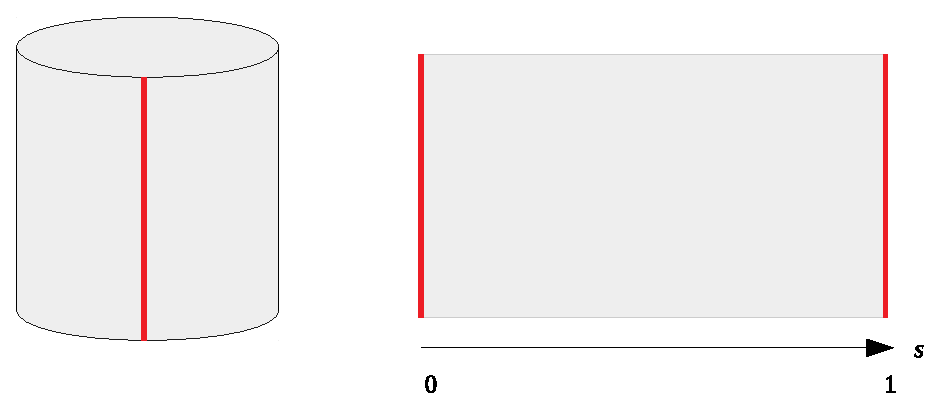
\includegraphics[width=.8\textwidth]{figures/cylinder_unwrap.eps}
    \caption{Unwrapping a cylinder. Vertices along seam (red line) require two texture coordinates}
    \label{fig:cylinder_unwrap}
\end{figure}


Hugues Hoppe \cite{hoppe1998efficient} presents a mesh representation where each face adjacent to a vertex can have different appearance attributes. The attribute values is associated with the corners of the faces instead of the vertices. A \emph{corner} is defined by Hoppe as a tuple $<vertex,face>$. The attribute values at a corner defines the value that should be used for face $f$ at vertex $v$. Corners with the same attributes and adjacent vertex are stored in a \emph{wedge}. The wedge has one or more corners and each vertex will be divided into one or more wedges. This representation is useful for simplification of meshes with discontinuities in their attribute fields. Discontinuities could result in a simplified mesh where adjacent faces have been separated which introduces new holes in the mesh.

\begin{figure}[ht]
    \centering
    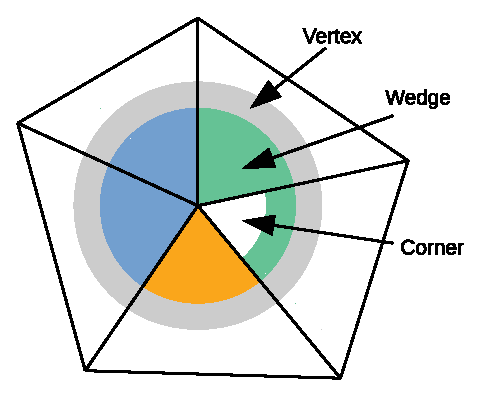
\includegraphics[width=.49\textwidth]{figures/wedge.eps}
    \caption{Vertex with wedges}
    \label{fig:wedge}
\end{figure}

%%%%%%%%%%%%%%%%%%%%%%%%%%%%%%%%%%%%%%%%%%%%%%%%%%%%%%%%%%%%%%%%%%%%%%
%%
%%% Metric for Appearance Preservation
%%
%%%%%%%%%%%%%%%%%%%%%%%%%%%%%%%%%%%%%%%%%%%%%%%%%%%%%%%%%%%%%%%%%%%%%%
\section{Metrics for Appearance Preservation} \label{sec:metrics_for_appearance_preservation}
Previously in \cref{sec:appearance-preserving_simplification,sec:progressive_meshes}, the metrics texture deviation and texture stretch have been defined. But to measure more exactly how much the visual appearance of a simplified mesh deviate from the original mesh another metric would be better. \emph{Lindstrom and Turk} \cite{lindstrom2000image} defines \emph{image-driven simplification} which captures images from different angles of the mesh. The difference between the images of the original and simplified mesh are computed in order to measure how well the appearance is preserved. This metric is more general and can be applied to all simplification algorithms since it only compares the original mesh to the simplified mesh.

The \emph{image metric} is defined as a function taking two images and gives the distance between them. To measure the distance the authors use root mean square of the luminance values of two images $Y^0$ and $Y^1$ with dimensions $m \times n$ pixels. It is defined as:
\begin{equation} \label{eq:rms_images}
  d_{RMS}(Y^0,Y^1) = \sqrt{\tfrac{1}{mn}\sum^m_{i=1}\sum^n_{j=1}(y^0_{ij} - y^1_{ij})^2}
\end{equation}

To evaluate the quality of the simplified mesh the authors capture images from 24 different camera positions. The positions are defined as the vertices of a rhombicuboctahedron which can be seen in \cref{fig:rhombicuboctahedron}. Two sets of $l$ images $Y^0 = {Y^0_h}$ and $Y^1 = {Y^1_h}$ with dimensions $m \times n$ is rendered and the RMS is then computed as:
\begin{equation}  \label{eq:rms_image_sets}
  d_{RMS}(Y^0,Y^1) = \sqrt{\tfrac{1}{lmn}\sum^l_{h=1}\sum^m_{i=1}\sum^n_{j=1}(y^0_{hij} - y^1_{hij})^2}
\end{equation}

\begin{figure}[h]
    \centering
    \includegraphics[width=0.25\textwidth]{figures/591px-Rhombicuboctahedron.jpg}
    \caption{Rhombicuboctahedron with 24 vertices which is used as the camera positions. 
      (\href{https://commons.wikimedia.org/wiki/File:Rhombicuboctahedron.jpg}{Rhombicuboctahedron} by Hellisp / \href{https://creativecommons.org/licenses/by/3.0/}{CC BY 3.0})}
    \label{fig:rhombicuboctahedron}
\end{figure}

\section{Measuring Algorithmic Performance} \label{sec:measuring_algorithmic_performance}

According to \emph{David Lilja}~\cite[p.~4]{lilja2005measuring}, there are three fundamental techniques that can be used when confronted with a performance-analysis problem: \emph{measurement}, \emph{simulation} or \emph{modeling}. While the book concentrates on evaluating computer performance, these techniques can also be applied when evaluating different algorithms. Measurement would be to actually execute the implemented algorithm and simultaneously gather interesting statistics (e.g. how long it took to finish and how much memory was needed), and use this to compare the algorithms. While modeling would be to analytically derive an abstract model for the algorithm (e.g. the Big \(\mathcal{O}\) worst-case running time and memory), and see which of them has a lower complexity.

Since not all of the algorithms in \cref{sec:related_work} have an analytical model derived by the authors, and also because the algorithms are to be evaluated in a real system, only the problems inherent to the measurement approach will be considered. One of the problems with doing measurements of a real system (a program running on a computer in this case), according to \emph{David Lilja}~\cite[p.~43]{lilja2005measuring}, is that they introduce noise. This noise needs to be modeled to be able to reach a correct conclusion, such as determining if algorithm A is faster than algorithm B. One way of doing this, according to \emph{David Lilja}~\cite[p.~48]{lilja2005measuring}, is to find the confidence interval of the measured value, by assuming the source's error is distributed according to some statistical distribution (like the Gaussian or the Student t-distribution). The confidence interval \([a,b]\) when assuming the source's error is t-distributed, can be found as shown below. Where \(n\) tests are taken (giving \(n-1\) degrees of freedom), with a significance level of \(\alpha\) (usually 5 \%).

\begin{equation} a = \overline{x} - t_k\frac{s}{\sqrt{n}}, \quad
   b = \overline{x} + t_k\frac{s}{\sqrt{n}}, \quad
t_k = t_{1-\alpha/2,n-1} \end{equation}

One common mistake, according to \emph{Schenker et al.}~\cite{schenker2001judging}, when using confidence intervals to determine if e.g. an implemented algorithm A is faster than B, is the use of the overlapping method to reach conclusions. If two confidence intervals \emph{do not} overlap, then the result is provably significant (that is, algorithm A is either faster or slower than B). However, the converse is not true, if two intervals \emph{do} overlap, then no conclusions can be reached since the result could be either significant or not significant.

%%%%%%%%%%%%%%%%%%%%%%%%%%%%%%%%%%%%%%%%%%%%%%%%%%%%%%%%%%%%%%%%%%%%%%
%%% theory.tex ends here

%%% Local Variables: 
%%% mode: latex
%%% TeX-master: "thesis"
%%% End: 

%%% lorem.tex --- 
%% 
%% Filename: lorem.tex
%% Description: 
%% Author: Ola Leifler
%% Maintainer: 
%% Created: Wed Nov 10 09:59:23 2010 (CET)
%% Version: $Id$
%% Version: 
%% Last-Updated: Wed Nov 10 09:59:47 2010 (CET)
%%           By: Ola Leifler
%%     Update #: 2
%% URL: 
%% Keywords: 
%% Compatibility: 
%% 
%%%%%%%%%%%%%%%%%%%%%%%%%%%%%%%%%%%%%%%%%%%%%%%%%%%%%%%%%%%%%%%%%%%%%%
%% 
%%% Commentary: 
%% 
%% 
%% 
%%%%%%%%%%%%%%%%%%%%%%%%%%%%%%%%%%%%%%%%%%%%%%%%%%%%%%%%%%%%%%%%%%%%%%
%% 
%%% Change log:
%% 
%% 
%% RCS $Log$
%%%%%%%%%%%%%%%%%%%%%%%%%%%%%%%%%%%%%%%%%%%%%%%%%%%%%%%%%%%%%%%%%%%%%%
%% 
%%% Code:

\chapter{Method} \label{cha:method}

    Now that the theoretical groundwork has been laid out, we describe in Section~\ref{sec:implementation} how the solution was implemented into Configuras graphics pipeline and then show how to evaluate it in Section~\ref{sec:evaluation} according to the posed research questions. In more detail, the implementation description shows how the different algorithms are implemented in practice and how these fit into Configura's pipeline. Moreover, we also show how the appearance evaluator has been implemented and integrated into the system, which provides a uniform way to simplify a mesh until a certain appearance threshold has been reached. In the evaluation part of the method, we describe how to measure the computation time, memory usage, polygon count and appearance preservation of a algorithm given a certain mesh and parameters. This method will thereafter be used to acquire the results needed to answer our research questions.

    \section{System Overview} \label{sec:system_overview}

    Before describing the system in detail, an overview is given in the Figure~\ref{fig:system_overview} below. In brief, the original mesh that is going to be simplified is given as input to the simplification algorithm, and as output comes a simpler mesh with less polygons. In order to provide a common interface to each of the algorithm's parameters, an appearance evaluator takes as input an appearance threshold (given as a RMS value) and the original and candidate meshes. This will provide the specific parameters to the algorithm in question, and incrementally reduce the quality measure (e.g. $|\mathcal{V}|$ or $\epsilon$) until the appearance threshold of a mesh candidate is satisfied.

    \begin{figure}[h]
        \centering
        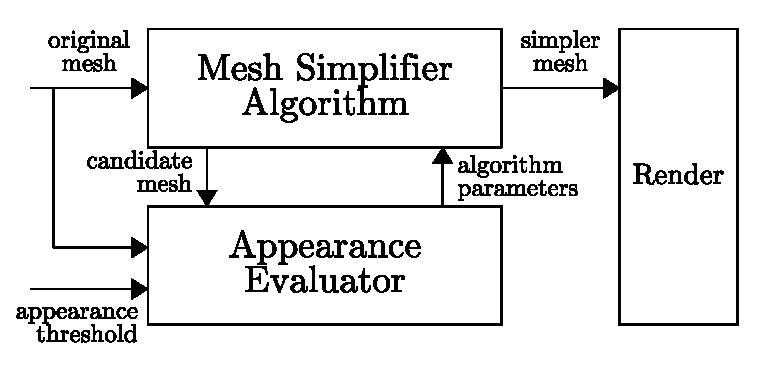
\includegraphics[width=0.55\textwidth]{figures/system_overview.eps}
        \caption{System Overview of a Simplifier Pipeline}
        \label{fig:system_overview}
    \end{figure}

    \section{Implementation} \label{sec:implementation}

    Before the chosen mesh simplification algorithm can be integrated into Configura's CET Designer, the three aforementioned different algorithms need to be implemented and evaluated. Only then can we make an informed decision on which of the algorithms are most suited for Configura, and thereafter integrate that solution into the CET Designer. In this section we describe how the three algorithms were implemented and the tools used to accomplish it. \textbf{Note:} for the course TDDD89 only a brief and preliminary overview is given over the implementation, since this part is best written after we've actually implemented some algorithms.

    The first step is to decide how and where to implement the simplification algorithms and the evaluation system. One possibility is to implement them directly in Configura's own language \emph{CM} (built in-house, a mix between C and Lisp). However, because we first only want to evaluate the algorithms without the overhead that may be introduced by CET Designer, this might not be the best idea. Therefore, we have decided to implement and evaluate the algorithms outside of CET Designer by building a simple testbed using C/C++ and the \emph{OpenGL} API (for evaluating the appearance and also to measure its rendering speed).

    To be able to change between the different algorithms, a common interface is implemented that can interact with the appearance evaluator. As can be seen in Figure~\ref{fig:system_overview}, the simplification algorithm takes a mesh and then gives a simplified mesh to the evaluator which will compare it to the original mesh. The simplification will be performed until a given appearance-threshold is reached (thus, giving all of the algorithms a universal stopping condition).

    A quick overview of how the algorithms work is explained in the theory chapter, and since the actual implementation is based on this description, only small details should deviate from the theory. But in order to give a more detailed description of how they are implemented, the practical details will also be described in the coming sections. However, as mentioned before, these sections will be mostly left empty at the moment since the implementations is not done yet for the scientific methods course. We then describe how to integrate the chosen solution.

        \subsection{Quadric-Based Error Metric} \label{sec:quadric-based_error_metric2}

        As a rule, the original mesh will be given as an ordinary triangle mesh (a so called ``triangle soup''), which is not suitable for applying the QEM algorithm (since the local neighborhood information isn't available). Instead, we convert this triangle soup to a half-edge mesh. This allows easy manipulation of the local neighborhood of the mesh, which is precisely what is needed when doing a edge collapse or when calculating the error quadrics of a given vertex.

        After doing this, the implementation basically follows the theoretical framework to the letter, where the least-cost edge is chosen to be contracted from the min-heap. Lastly, this edge is collapsed and then the remaining ``hole'' is simply (but with a few special cases...) linked back together so that the local neighborhood of the vertex still qualifies as a closed manifold. All source code is provided at the end of this report (\textbf{not} for the TDDD89 course).

        \subsection{Appearance-Preserving Simplification} \label{sec:appearance-preserving_simplification2}

        \subsection{Texture Mapped Progressive Meshing} \label{sec:texture_mapped_progressive_meshing2}

        \subsection{Integrating Solution into the Pipeline} \label{sec:integrating_solution_into_the_pipeline}

        When the candidate algorithm has been chosen, it has to be integrated into CET Designer. Since we've chosen to evaluate the solution in C/C++ in our own renderer, the algorithm needs to be ported to the Configura CM language. It also needs to interact with the existing file format of the models, which means that either an existing Configura library will be needed or a custom one will need to be written for our purposes. After that, the integration is mostly painless, because the algorithm doesn't depend that much on any of the other parts in CET Designer. It should just be a case of: \emph{original mesh} $\rightarrow$ \emph{mesh simplifier} $\rightarrow$ \emph{simplified mesh}.

    \section{Evaluation} \label{sec:evaluation}

        In order to determine which of these algorithms provide the best performance for a target appearance threshold, an evaluation of the polygon count, computation time, memory usage and rendering time of the simplified mesh is done for each of the implemented solutions. In the results from this step, a series of tables are generated to compare the performance between the algorithms by using a common comparison framework. In this section, we describe this common comparison framework and then show how we can measure each of the parameters.

        In essence, this is done by targeting a certain appearance threshold, tweaking the mesh simplification algorithm's parameters to achieve this threshold, and then measuring the given performance. This gives a universal measure of ``quality'' for all of the algorithms, which would otherwise have different error metrics used for applying the simplification. Since the performance measures are noisy, a total of \(n=20\) samples will be taken. According to \emph{David Lilja}~\cite[p.~50]{lilja2005measuring} the t-student distribution should be used when \(n < 30\), as shown in Section~\ref{sec:measuring_algorithmic_performance}.

        The pack of test meshes that are going to be used in the comparison are a combination of textured models provided by Configura and others taken from the public domain. The exact selection of these is still to be decided, but should include both low- \& high-polygon meshes.

        \subsection{Appearance Preservation} \label{sec:appearance_preservation}
        In order to compare the appearance preservation of the mesh simplification algorithms, the image-metric explained in section~\ref{sec:metrics_for_appearance_preservation} is used. It is useful since it can compare the difference of any two meshes, therefore, it does not depend on the algorithm used.

        For both the original mesh and a simplified mesh, 24 images with resolution $512 \times 512$ is rendered with a simple renderer based on \emph{OpenGL}. The camera is placed at the vertices of a rhombicuboctahedron and is faced towards the center where the mesh is placed. A light source is placed at the camera position. This will make sure that the surface facing the camera will be illuminated.

        The two sets of 24 images each is used to compute the RMS of the simplified mesh with equation~\ref{eq:rms_image_sets}. This RMS value can then be used to compare how well the algorithms perform. 
        \subsection{Polygon Count} \label{sec:polygon_count}
        Concerning research question 3, the appearance preservation for a specific target polygon count needs to be measured. Therefore, the simplification algorithms is tasked to simplify until the target polygon count is reached. When it is reached, the image-metric is used to measure how well the appearance is preserved. Measurements will be performed for multiple target polygon counts. 

        \subsection{Computation Time} \label{sec:computation_time}

        An important property of a mesh simplification algorithm is the time it takes to simplify a full-resolution mesh to a lower-resolution mesh. While this doesn't impact the run-time of the mesh (that is accounted for by the rendering time, measured in Section~\ref{sec:rendering_time}), it is still important to reduce it as much as possible. This is especially true if the LoD is dynamically generated at run-time, but it is also important since many more meshes can be simplified per time unit (important if a simplifier is to be provided as a service, as \emph{Simplygon Linköping} does).

        In order to compare the execution time of the different algorithms, they all target the same appearance thresholds as specified in Section~\ref{sec:appearance_preservation} by tweaking the parameters unique to each algorithm. We then measure the time it takes for the simplification algorithm to execute when using these parameters, in other words, simply by: \(time_\mathcal{A} = end_\mathcal{A} - start_\mathcal{A}\) for an algorithm \(\mathcal{A}\). Of course, this measurement is done several times to account for noise. After calculating the mean \(\bar{x}\) and the standard-deviation \(s\), one can find the confidence interval \([a, b]\) of the execution time by the equations shown in Section~\ref{sec:measuring_algorithmic_performance} with 19 degrees of freedom and \(\alpha = 5 \%\).

        \subsection{Memory Usage} \label{sec:memory_usage}

        Another important performance property of the algorithm is the accumulated memory used when simplifying the mesh. Depending on the size of the mesh in triangles, the algorithm could consume large amounts of memory (and might not even fit in the primary memory in some cases). It is therefore important to compare the simplification algorithms to determine those which are suited for optimizing large triangle meshes and those that aren't. Since this measure will always be deterministic (at least for the method we use to measure it), there is no need to apply any statistical measures. The \emph{Valgrind} suite was chosen since it has the \emph{Massif} heap profiler, which gives accurate memory usage. According to the \emph{Massif documentation}~\cite{valgrind2017manual} there is an expected slowdown of 20x, which isn't a problem since the computation time and rendering time are measured separately. Below are the commands to find the memory usage.

        \begin{lstlisting}[language=bash]
 (*\textbf{valgrind}*) --tool=massif (*\textit{./simplify --algorithm=<algorithm> <input-mesh> <output-mesh>}*)
        \end{lstlisting}

        \subsection{Rendering Time} \label{sec:rendering_time}
        One main purpose of simplifying a mesh is to reduce the rendering time. Therefore, the frame rate is measured when rendering the original mesh and the simplified meshes. The simplified meshes comes from the previous steps where different appearance-thresholds was targeted. Frame rate is measured by counting how many frames that have been rendered during a period of one second. As with computation time, this measurement may have noise and therefore multiple samples needs to be obtained. The mean and condifidence interval is obtained in the same way.

%%%%%%%%%%%%%%%%%%%%%%%%%%%%%%%%%%%%%%%%%%%%%%%%%%%%%%%%%%%%%%%%%%%%%%
%%% method.tex ends here

%%% Local Variables: 
%%% mode: latex
%%% TeX-master: "thesis"
%%% End: 

\chapter{Results} \label{cha:results}
TODO: Overview of results chapter.

% 800 Office woman

\iffalse
\begin{figure}[h]
  \centering
  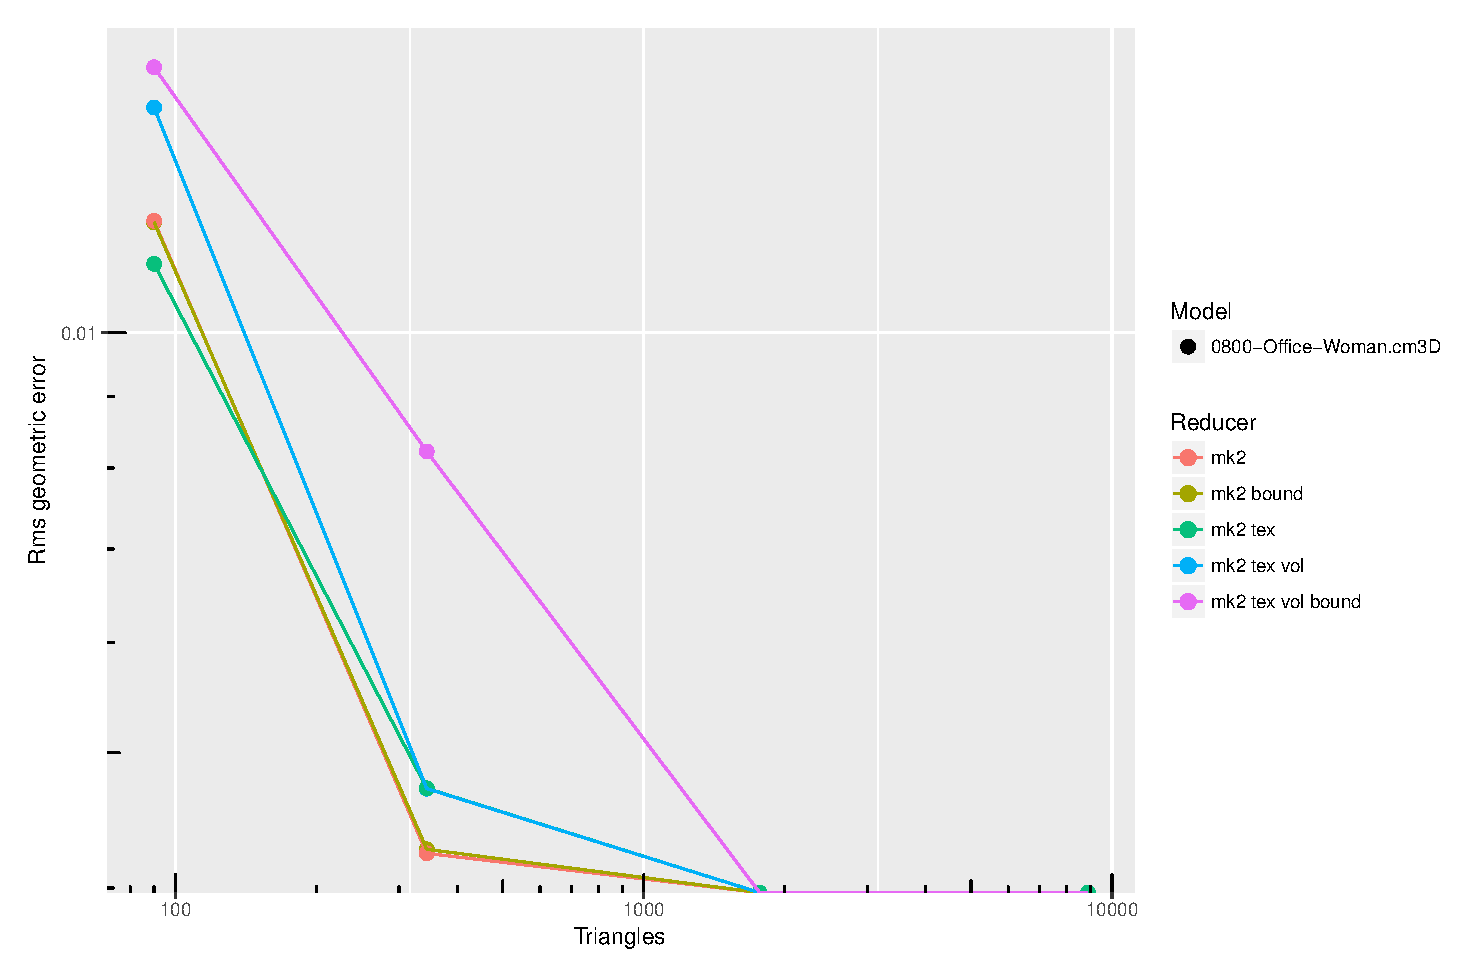
\includegraphics[width=\textwidth]{figures/Rdata/geometric_800.eps}
  \caption{Rms geometric error of ``office woman'' model}
  \label{fig:woman_geometric_error}
\end{figure}


\begin{figure}[h]
  \centering
  \includegraphics[width=\textwidth]{figures/Rdata/color_800.eps}
  \caption{Rms color error of ``office woman'' model}
  \label{fig:woman_color_error}
\end{figure}
\fi

\section{RMS luminance error}
RMS luminance error was computed by rendering multiple images of a model from multiple angles and can be seen in \cref{fig:mean_luminance_error}. Four LoD:s are presented where \emph{super} have the most amount of triangles and \emph{low} have the least amount of triangles. The error was measured for different settings of seam and volume preservation.

\begin{figure}[h]
  \centering
  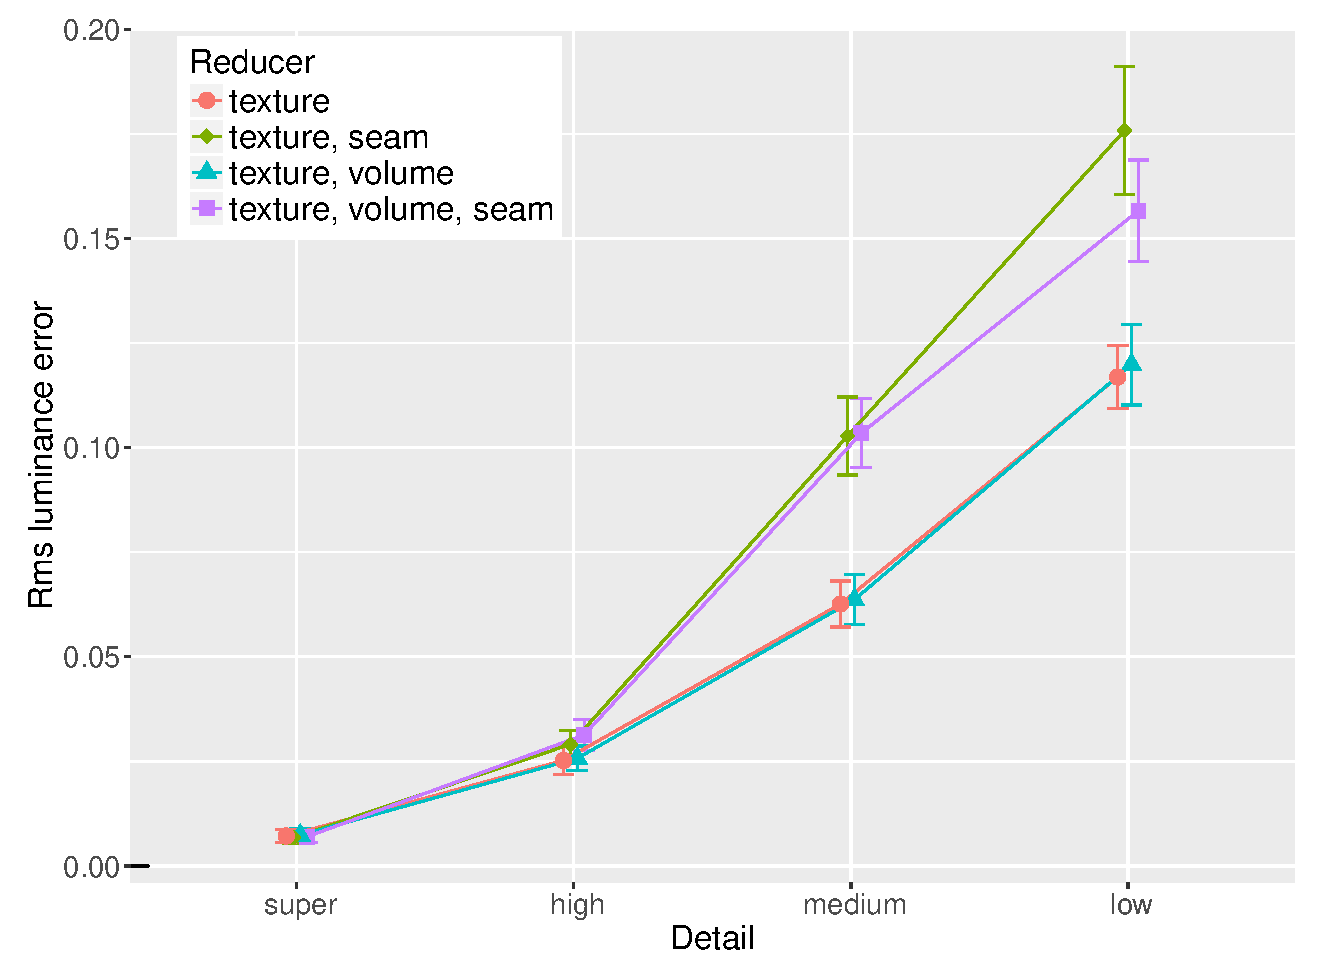
\includegraphics[width=\textwidth]{figures/Rdata/rms_luminance.eps}
  \caption{Rms luminance error}
  \label{fig:mean_luminance_error}
\end{figure}

\section{Hausdorff distance}

\section{Improved Texture}
A pull-push algorithm was implemented in order to improve the texture that is used by a mesh since undefined areas may be used. Given a texture (\cref{fig:original_texture_atlas}), rays are casted for each pixel in order to generate a black and white image. Valid pixels get a white color and invalid pixels a black color as seen in \cref{fig:valid_pixels}. Pixels with a corresponding black pixel will be filled in by the pull-push algorithm. This will result in the texture seen in \cref{fig:improved_texture} where all the empty pixels have been filled in.

\begin{figure}[h]
  \centering
  \begin{subfigure}[b]{.3\textwidth}
    \includegraphics[width=\textwidth]{figures/woman_input.jpg}
    \caption{Original}
    \label{fig:original_texture_atlas}
  \end{subfigure}
  ~
  \begin{subfigure}[b]{.3\textwidth}
    \includegraphics[width=\textwidth]{figures/woman_bound.png}
    \caption{Valid pixels}
    \label{fig:valid_pixels}
  \end{subfigure}
  ~
  \begin{subfigure}[b]{.3\textwidth}
    \includegraphics[width=\textwidth]{figures/woman_output.png}
    \caption{Improved texture}
    \label{fig:improved_texture}
  \end{subfigure}
  \caption{Filling in empty pixels in the texture atlas}
  \label{fig:improve_texture_atlas}
\end{figure}

Simplification of the office woman model introduce some black areas where the original seam used to be (\cref{fig:using_original_texture}). The same model have also been rendered with the new improved texture (\cref{fig:using_improved_texture}) to give a better appearance.

\begin{figure}[h]
  \centering
  \begin{subfigure}[b]{.2\textwidth}
    \includegraphics[width=\textwidth]{figures/woman_render.png}
    \caption{Using original texture}
    \label{fig:using_original_texture}
  \end{subfigure}
  \qquad
  \begin{subfigure}[b]{.2\textwidth}
    \includegraphics[width=\textwidth]{figures/woman_render_improved.png}
    \caption{Using improved texture}
    \label{fig:using_improved_texture}
  \end{subfigure}
  \caption{Mesh using original and improved texture}
  \label{fig:texture_comparison}
\end{figure}

% super:  8886
% high:   1768
% medium: 344
% low:    90

\begin{figure}[h]
  \centering
  \begin{subfigure}[b]{.22\textwidth}
    \includegraphics[width=\textwidth]{figures/woman/cropped/0.png}
    \caption{super}
    \label{fig:woman0}
  \end{subfigure}%\qquad
  \begin{subfigure}[b]{.22\textwidth}
    \includegraphics[width=\textwidth]{figures/woman/cropped/1.png}
    \caption{high}
    \label{fig:woman1}
  \end{subfigure}
  \centering
  \begin{subfigure}[b]{.22\textwidth}
    \includegraphics[width=\textwidth]{figures/woman/cropped/2.png}
    \caption{medium}
    \label{fig:woman2}
  \end{subfigure}%\qquad
  \begin{subfigure}[b]{.22\textwidth}
    \includegraphics[width=\textwidth]{figures/woman/cropped/3.png}
    \caption{low}
    \label{fig:woman3}
  \end{subfigure}
  \caption{Office woman LoD:s}
  \label{fig:woman_lod}
\end{figure}


\begin{figure}[h]
  \centering
  \begin{subfigure}[b]{.22\textwidth}
    \includegraphics[width=\textwidth]{figures/woman/equal_distance/0.png}
    \caption{super}
    \label{fig:womaneq0}
  \end{subfigure}%\qquad
  \begin{subfigure}[b]{.22\textwidth}
    \includegraphics[width=\textwidth]{figures/woman/equal_distance/1.png}
    \caption{high}
    \label{fig:womaneq1}
  \end{subfigure}
  \centering
  \begin{subfigure}[b]{.22\textwidth}
    \includegraphics[width=\textwidth]{figures/woman/equal_distance/2.png}
    \caption{medium}
    \label{fig:womaneq2}
  \end{subfigure}%\qquad
  \begin{subfigure}[b]{.22\textwidth}
    \includegraphics[width=\textwidth]{figures/woman/equal_distance/3.png}
    \caption{low}
    \label{fig:womaneq3}
  \end{subfigure}
  \caption{Office woman LoD:s}
  \label{fig:woman_lodeq}
\end{figure}

\chapter{Discussion} \label{cha:discussion}
This chapter provides a discussion on the work. First, a discussion of the results is given in \cref{sec:discussion_results}. Afterwards, in \cref{sec:discussion_method} the used method is discussed.

\section{Results} \label{sec:discussion_results}

\subsection{Luminance Error} \label{sec:discussion_luminance}
When simplifying a mesh to be used for LoD super and high, considering the seam or the volume does not affect the rms luminance error much as can be seen in \cref{fig:mean_luminance_error}. At the high level the graphs start to diverge but the confidence intervals overlap which means that we can not say with any significance that any setting is better than another. However, for medium and low, considering the seam gives a worse result than not considering it.

Not allowing all edge removals in the seam constrains the simplification and this affects the final geometry. Geometry that differs a lot from the original will give a high luminance error. This occurs since in some areas of the rendered images the background is rendered where the mesh used to be. In this case the background was white leading to a high difference of the images.

Ignoring the seam for now, if the volume is considered the error becomes slightly larger but not with any significance. Not considering the volume may be a better choice since the optimization problem would be less constrained and could be solved faster.

\subsection{Color and Geometric Error} \label{sec:discussion_color_geom}
To further investigate when the seam and volume should be considered points was sampled on the surfaces of the mesh. A comparison of this can be seen in \cref{fig:geo_col_error}.

If we first look at the geometric error the two highest LoD:s have a geometric error close to zero for all settings. For the other two lower levels we can see, just as discussed in \cref{sec:discussion_luminance}, that the seam preservation give a worse result. According the graphs of the geometric error the best setting would be to only consider the texture.

When looking at the color error the difference is small between the settings. However, the rms color error for the super LoD is lower when the seam is considered. Therefore, considering the seam may give a better result for the super and high LoD since the geometric error was small.



\subsection{Volume Preservation} \label{sec:discussion_volume}
\cref{fig:volume_diff} shows how the volume of meshes is affected by different configurations of texture, seam and volume preservation. Just as discussed in previous sections the configuration affect the result for the two highest LoD:s very little. By looking at the figure we can see that the volume constraint indeed keep the volume better. Considering the seam gives a larger difference in volume but it is kept better if the volume is also consider. The best configuration if one wants to keep the volume is to only consider the texture and the volume.


\subsection{Improved Texture Atlas} \label{sec:discussion_texture}
As we have seen from the graphs the seam gives a bad result in terms of luminance error and geometric error. But, when the seam is not considered undefined areas of the texture may appear just at the seam. This can be seen in \cref{fig:using_original_texture} where where black areas have appeared on the legs of the model.

Using the pull-push algorithm to fill in missing pixel values results in a new texture that gives a better result in the seams. As can be seen in \cref{fig:using_improved_texture} almost all the black areas have disappeared from the legs. However, on the left leg a small hint of black can be seen. By looking at the new texture we can see that there still remains some black areas just at the seam bound.

\subsection{Comparison of LoD:s} \label{sec:discussion_lod}
Looking at the four LoD:s of the office woman model in \cref{fig:woman_lodeq} we can see how the different levels are affected by simplification. The super and high have not changed very much the the appearance is still good. One can see that the silhouette of the high LoD is not as round as the super LoD. For medium the effect of the simplification is clear and even more for the low LoD where we can clearly see the triangles.

When looking at the LoD:s from the distance where they would actually be used the edgy silhouette is harder to distinguish. 

\section{Method} \label{sec:discussion_method}

  
  %%%
  % N/A for this work
  %%%
%\section{The work in a wider context} \label{sec:work_in_a_wider_context}

\chapter{Conclusion} \label{cha:conclusion}
 TODO: Overview of conclusion chapter.

\printbibliography

\end{document}

%%%%%%%%%%%%%%%%%%%%%%%%%%%%%%%%%%%%%%%%%%%%%%%%%%%%%%%%%%%%%%%%%%%%%%
%%% demothesis.tex ends here

